\documentclass[]{beamer}
\usepackage{verbatim}
\usepackage{xcolor}
\usepackage{multirow}
\usepackage{amssymb}
\usepackage{tikz}
\usepackage{hyperref}
\usetikzlibrary{positioning,fit}
%\usepackage{enumitem}
\usetheme{Warsaw}
\setbeamertemplate{navigation symbols}{}
\newcommand{\blue}[1]{{\color{blue} #1}}
\newcommand{\red}[1]{{\color{red} #1}}
\newcommand{\grn}[1]{{\color{green} #1}}
\newcommand{\bluRed}[2]{{\color{blue} #1}{\color{red} #2}}
\newcommand{\qtns}[0]{\begin{center} Questions? \end{center}}
\newcommand{\nl}[1]{\vspace{#1 em}}
\newcommand{\cntrImg}[2]{\begin{center}\includegraphics[scale=#2]{#1}\end{center}}
\newcommand{\defn}[1]{{\bf #1}}
\let\emptyset\varnothing
\newcommand{\SampS}[0]{$\mathcal{S}$}

\title{Math 3070, Applied Statistics}

\begin{document}
\begin{frame}
    \begin{beamercolorbox}[rounded=true,wd=\textwidth,center]{title}
        \usebeamerfont{title}\inserttitle
    \end{beamercolorbox}
    \begin{center}
        Section 1\\
        \nl{0.5}
        September 27, 2019
    \end{center}
\end{frame}
\begin{frame}{Lecture Outline, 9/27}
    Section 4.4
    \begin{itemize}
        \item Exponential Random Variable
        \item Chi-Squared ($\chi^2$) Random Variable
        \item Gamma Random Variable
    \end{itemize}
\end{frame}
\begin{frame}{Exponential Random Variable}
    \begin{block}{}
        We say that $X$ is an \textbf{exponential} random variable with rate $\lambda>0$ if $X$ has pdf
        $$f(x) = \begin{cases}\lambda e^{-\lambda x} & \text{if }x\geq 0 \\ 0 & \text{if }x<0\end{cases}$$
        $X \sim exp(\lambda)$
    \end{block}
    \pause We can check that this is a valid pdf:

    \begin{tabular}{p{5.5cm}p{4cm}}
        \vspace{0cm}
        $\begin{aligned}[t]
                \int_{-\infty}^\infty f(x)\ dx & = \int_0^\infty \lambda e^{-\lambda x}\ dx                      \\
                                               & = \lambda \frac{-1}\lambda e^{-\lambda x}\Big\vert_{x=0}^\infty \\
                                               & = 0 - (-1) = 1
            \end{aligned}$
         &
        \vspace{-.25cm}
        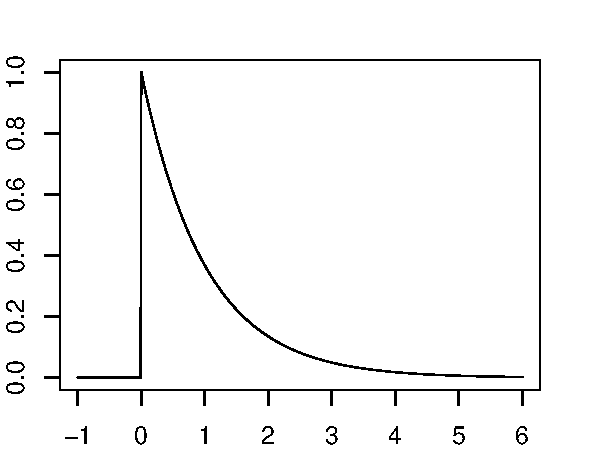
\includegraphics[scale=.55]{ch4_pdf_exp.pdf}
    \end{tabular}
\end{frame}
\begin{frame}{CDF of Exponential Random Variable}
    Recall the pdf of an exponential random variable $x$ with rate $\lambda$ is
    $$f(x) = \begin{cases}\lambda e^{-\lambda x} & \text{if }x\geq 0 \\ 0 & \text{if }x<0\end{cases}$$
    \pause The cdf $F(x)$ is therefore, for $x\geq 0$,
    \begin{align*}
        F(x) & =\int_{-\infty}^x f(t)\ dt=\int_0^x \lambda e^{-\lambda t}\ dt \\
             & = -e^{-\lambda t}\big\vert_{t=0}^x = 1-e^{-\lambda x}
    \end{align*}
    $$Fx) = \begin{cases}\lambda 1-e^{-\lambda x} & \text{if }x\geq 0 \\ 0 & \text{if }x<0\end{cases}$$
\end{frame}
\begin{frame}{Exponential Waiting Times}
    Consider a Poisson Random Variable with rate $\lambda$.
    \begin{itemize}
        \item Let $Y_t$ be the number of events occurring in the interval $[0,t]$.
              \pause \item So $Y_t$ is a Poisson random variable with mean $\lambda t$.
              \pause \item Let $X$ be the time of the first event.
    \end{itemize}
    \begin{align*}
        P(X \leq t)   & = P(\text{first event occurs by time $t$})                                             \\
        \uncover<4->{ & = P(\text{at least one event occurs in the interval $[0,t]$})\\}
        \uncover<5->{ & = P(Y_t \geq 1) \\}
        \uncover<6->{ & = 1- P(Y_t = 0) \\}
        \uncover<7->{ & = 1 - \frac{e^{-\lambda t}(-\lambda t)^0}{0!} \\}
        \uncover<8->{ & = 1 - e^{-\lambda t}}
    \end{align*}
    \uncover<9->{This is the cdf of an exponential random variable of rate $\lambda$. Therefore, in a Poisson process, the waiting time for the first event is an exponential random variable with rate $\lambda$.}
\end{frame}
\begin{frame}{Mean of Exponential}
    Using integration by parts, we can find the mean of an exponential random variable $X$ of rate $\lambda$:
    \begin{align*}
        E(X)          & =\int_{-\infty}^\infty xf(x)\ dx                                                                  \\
        \uncover<2->{ & =\int_0^\infty x\lambda e^{-\lambda x}\ dx \\}
        \uncover<3->{ & = -xe^{-\lambda x}\big\vert_0^\infty + \int_0^\infty e^{-\lambda x}\ dx \\}
        \uncover<4->{ & = 0 - 0 - \frac1{\lambda}e^{-\lambda x}\big\vert_0^\infty = \frac 1\lambda}
    \end{align*}

\end{frame}
\begin{frame}{Variance of Exponential Distribution}
    We can find the variance of an exponential random variable $X$ by using integration by parts twice:
    \pause\begin{align*}
        E(X^2)        & =\int_0^\infty x^2\cdot\lambda e^{-\lambda x}\ dx                                                                                                 \\
        \uncover<3->{ & = -x^2 e^{-\lambda x}\big\vert_0^\infty-\int_0^\infty -2xe^{-\lambda x}\ dx \\}
        \uncover<4->{ & = 2\int_0^\infty xe^{-\lambda x}\ dx \\}
        \uncover<5->{ & = 0-0+2\left[-\frac1\lambda xe^{-\lambda x}\big\vert_0^\infty - \int_0^\infty -\frac1\lambda e^{-\lambda x}\ dx \right] \\}
        \uncover<6->{ & = 2\left[0-0-\frac1{\lambda^2}e^{-\lambda x}\big\vert_0^\infty\right] = \frac2{\lambda^2}}
    \end{align*}
    \uncover<7->{So $V(X)=E(X^2)-[E(X)]^2 = \frac2{\lambda^2} - \left(\frac1\lambda\right)^2=\frac1{\lambda^2}$.
    In other words, the standard deviation is $\sigma=1/\lambda=\mu$.}
\end{frame}
\begin{frame}{Memoryless Property of Exponential}
    The exponential distribution is useful for modeling the lifetime of components where breakdowns are the result of sudden, random failures rather than gradual deterioration.

    \vspace{.2cm}\pause In general, an exponential random has the ``memoryless" property:
    \begin{block}{}
        \vspace{-.2cm}$$P(X\geq s+t \mid X\geq s) = P(X\geq t)$$
    \end{block}

    \vspace{.25cm}
    \pause Proof: $\begin{aligned}[t]
            P(X\geq s+t\mid X\geq s) & = \frac{P(X\geq s+t \cap X\geq s)}{P(X\geq s)} \\
                                     & = \frac{P(X\geq s+t)}{P(X\geq s)}              \\
                                     & = \frac{e^{-\lambda(s+t)}}{e^{-\lambda s}}     \\
                                     & = e^{-\lambda t} = P(X\geq t)
        \end{aligned}$\\
    Due to the memoryless property, the exponential distribution can model times between events of a Poisson Random Variable.
\end{frame}
\begin{frame}{Example}
    \begin{block}{}
        Suppose that the lifetime $X$ of a lightbulb follows an exponential distribution with mean $\mu=100$ days. What is the probability that the lifetime is at least 50 days?
    \end{block}

    \pause \vspace{.2cm}Solution: The rate of failure is $\lambda = 1/\mu = 1/100$ per day. Therefore,
    \begin{align*}
        P(X \geq 50)  & = \int_{50}^{\infty} \lambda e^{-\lambda x}\ dx                    \\
        \uncover<3->{ & = -e^{-\lambda x}\big\vert_{50}^{\infty} \\}
        \uncover<4->{ & = e^{-50\lambda} \\}
        \uncover<5->{ & = e^{-50/100} = e^{-1/2} \approx .607}
    \end{align*}

    \pause \vspace{-.2cm}
    \uncover<6->{\begin{block}{}
            In general, if $X$ is an exponential random variable with rate $\lambda$,
            $$P(X \geq t)=e^{-\lambda t}$$
        \end{block}}
\end{frame}
\begin{frame}{Example}
    \begin{block}{}
        Again suppose that the lifetime $X$ of a lightbulb follows an exponential distribution with mean $\mu=100$ days. Given that the bulb has survived for 30 days, what is the probability that it will last for at least 50 more?
    \end{block}
    \vspace{-.2cm}\pause \begin{align*}
        P(X\geq80 \mid X\geq 30) & = \frac{P(X\geq 80 \cap X\geq 30)}{P(X\geq 30)}                   \\
        \uncover<3->{            & = \frac{P(X\geq 80)}{P(X\geq 30)} \\}
        \uncover<4->{            & = \frac{e^{-80\lambda}}{e^{-30\lambda}} \\}
        \uncover<5->{            & = e^{-50\lambda} = e^{-50/100}=e^{-1/2} \approx .607}
    \end{align*}
    \uncover<6->{This is the same as the probability of a new bulb lasting 50 days, as we calculated on the previous slide.}
\end{frame}
\begin{frame}{Summary}
    \begin{itemize}
        \item $X\sim exp(\lambda)$ means $X$ follows an exponential distribution with parameter $\lambda$.
        \item Poisson models number of events with rate $\lambda$. Exponential with the same $\lambda$ models wait times between them.
        \item Memoryless property is a subtle modeling issue, but mathematical nice.
        \item PDF:
              $$f(x) = \begin{cases}\lambda e^{-\lambda x} & \text{if }x\geq 0 \\ 0 & \text{if }x<0\end{cases}$$
        \item CDF:
              $$Fx) = \begin{cases}\lambda 1-e^{-\lambda x} & \text{if }x\geq 0 \\ 0 & \text{if }x<0\end{cases}$$
        \item $$ E[X] = \frac{1}{\lambda} \hskip 2em Var(X) = \frac{1}{\lambda^2} $$
    \end{itemize}
\end{frame}

\begin{frame}{Chi-squared Random Variable}
    If $Z$ is a standard normal random variable, then $Z^2$ has a so-called \textbf{chi-squared} distribution with one \textbf{degree of freedom}.

    \begin{block}{}
        A \textbf{chi-square} random variable with $\nu>0$ degrees of freedom has pdf
        $$f(x) = \begin{cases}\frac1{2^{\nu/2}\Gamma(\nu/2)}x^{\nu/2-1}e^{-x/2},& x\geq 0 \\ 0, & x<0\end{cases}$$
        $X \sim \chi^2(\nu)$
    \end{block}
    Since $Z$ is important in the central limit theorem, one should expect that $\chi^2$ will appear in many applications.
    $$\Gamma(k) = \int_0^\infty x^{k-1}e^{-x}\ dx$$
\end{frame}
\begin{frame}{Chi-squared Random Variable, $Z^2$ Explained}
    Consider $Z\sim N(0,1)$. Compute the pdf of $X= Z^2$.
    For $x<0$, $ P(Z^2<0)=0$.
    Consider $x>0$.
    \pause
    \begin{align*}
        P(Z^2<x) & = P(-\sqrt{x}<Z \sqrt{x})                                                             \\
                 & = \int_{-\sqrt{x}}^{\sqrt{x}} \frac{1}{\sqrt{2\pi}} \exp\bigg(\frac{-y^2}{2}\bigg) dy \\
                 & = 2 \int_{-\infty}^{\sqrt{x}} \frac{1}{\sqrt{2\pi}} \exp\bigg(\frac{-y^2}{2}\bigg) dy
    \end{align*}
    \pause Last step uses symmetry of the distribution. Differentiate in $x$ to recover the PDF.
    \pause
    \begin{align*}
        \frac{d}{dx} P(Z^2 < x) & = \frac{2}{\sqrt{2\pi}}\exp\bigg(\frac{-x}{2}\bigg)\frac{1}{2\sqrt{x}} = \frac{1}{\sqrt{2\pi}}\frac{1}{\sqrt{x}}\exp\bigg(\frac{-x}{2}\bigg) \\
    \end{align*}
    Observe this is the PDF of a $\chi^2(1)$ random variable.
\end{frame}
\begin{frame}{Chi-squared Random Variable, Mean and Variance}
    Consider $X\sim \chi^2(\nu)$.
    $$E[X] = \nu$$
    $$ V(X) = 2\nu $$
    \vfill
\end{frame}
\begin{frame}{Gamma Distribution}
    \begin{block}{}
        A \textbf{gamma} random variable $X$ with parameters $\alpha,\beta>0$ is given by the pdf
        $$f(x) = \begin{cases}\frac{1}{\beta^\alpha\Gamma(k)}x^{\alpha-1}e^{-x/\beta}, & x\geq 0 \\ 0, & x<0\end{cases}$$
        $X\sim \Gamma(\alpha,\beta)$ \\ \nl{0.5}
        $\beta=1$ is called the standard gamma.
    \end{block}
    Used to relate other random variables together. For example, a $\Gamma(\nu/2,2)$ and $\chi^2(\nu)$ have the same PDFs.
    \\ \nl{0.5}
    These relationships allows us to relate their parameters.
\end{frame}
\begin{frame}{Gamma Distribution, Mean and Variance}
Consider $X \sim \Gamma(\alpha,\beta)$
$$ E[X] = \alpha\beta $$
$$ V(X) = \alpha\beta^2 $$
\pause Check to see that the mean and standard deviation of the $\chi^2$ are reproduced with $\alpha=\nu/2$ and $\beta = 2$.
\pause $$E[X] = \alpha\beta = \frac{\nu}{2} 2 = \nu$$
\pause $$ V(X) = \alpha\beta^2 = \frac{\nu}{2} 2^2 = 2 \nu$$
\vfill
\end{frame}
\begin{frame}{Summary}
    \begin{block}{}
        $X \sim \chi^2(\nu)$ with $\nu>0$\\
        PDF:
    $$f(x) = \begin{cases}\frac1{2^{\nu/2}\Gamma(\nu/2)}x^{\nu/2-1}e^{-x/2},& x\geq 0 \\ 0, & x<0\end{cases}$$
        $$ E[X]  = \nu \hskip 2em V(X) = 2\nu $$
    \end{block}
    \begin{block}{}
        $X \sim \Gamma(\alpha,\beta)$ with $\alpha,\beta>0$\\
        PDF:
    $$f(x) = \begin{cases}\frac{1}{\beta^\alpha\Gamma(k)}x^{\alpha-1}e^{-x/\beta}, & x\geq 0 \\ 0, & x<0\end{cases}$$
        $$ E[X]  = \alpha\beta \hskip 2em V(X) = \alpha\beta^2 $$
    \end{block}
    \begin{itemize}
        \item $Z\sim N(0,1) \to Z^2 \sim \chi^2(1)$
        \item $X\sim \Gamma(\nu/2,2)  \iff X \sim \chi^2(\nu)$
        \item More relations between random variables to come.
    \end{itemize}
\end{frame}
\end{document}